\subsection{Passivity Analysis}
The stability analysis of the system gives information about the region of stability of the proposed controller. The passivity is analyzed by observing the evolution of the kinetic energy of the system, which is given as:
\begin{equation}
	W(\vecs \xi, \vecs{\dot \xi}) = \frac{1}{2}  \dot{\vecs{\xi}}^T \matd{M}(\vecs \xi) \dot{\vecs{\xi}} \label{eq:energy_system}
\end{equation}

\begin{lemma} \label{lemma:passivity}
  % Let $\vect f(\vecs \xi)$ be the desired velocity with bounded magnitude, i.e., $\| \vect f(\xi) \| < \infty, \forall \xi \in \mathbb{R}^N$.
   Let us assume a robotic system as described in \eqref{eq:robot_dynamics} is controlled using \eqref{eq:control_command} using the damping matrix $\matd D(\vecs \xi)$ given in \eqref{eq:damping_summation} with damping values $s_i = 1$.
   The system is passive with respect to the input-output pair $\vecs \xi_e$, $\vecs{\dot \xi}$ when exceeding the desired velocity $\vect f(\vecs \xi)$ , i.e., $\dot{W} \leq \vecs{\dot \xi}^T \vecs \tau^e, \; \forall \vecs \xi \in \mathbb{R}^N: \| \vecs{\dot \xi} \| \geq \| \vect f(\vecs \xi) \|$ and the storage function being the kinetic energy $W \in \mathbb{R}$ given in \eqref{eq:energy_system}
\end{lemma}

\begin{proof}
The time derivative of storage function $W$ can be evaluated as:
\begin{align}
  % \begin{split}
    \dot W(\vecs \xi, \vecs{\dot \xi}) &=
    \vecs{\dot \xi}^T \matd M(\vecs \xi) \vecs{\ddot \xi}  + \frac{1}{2} \vecs{\dot \xi}^T \dot{\matd M}(\vecs \xi) \vecs{\dot \xi}  \nonumber \\
  &= \frac{1}{2} \vecs{\dot \xi}^T \left( \dot{\matd M}(\vecs \xi) - 2 \matd C(\vecs \xi) \right) \dot{\vecs \xi} - \vecs{\dot \xi}^T \matd{D}(\vecs \xi) \vecs{\dot \xi} + \vecs{\dot \xi}^T \vecs \tau^e \nonumber \\
  &= - \vecs{\dot \xi}^T \matd{D}(\vecs \xi) \left( \vecs{\dot\xi} - \mathbf{f}(\vecs \xi) \right) + \vecs{\dot\xi}^T \tau^e
  % \end{split}
\end{align}
where we use the fact that $\dot{\matd M} - 2 \matd C$ is skew-symmetric, and hence the corresponding summand is zero.

% \subsubsection{Stability with Uniform Damping}
Let us investigate the region where the passivity holds. From the Lemma, we assume that all damping values are equal to one, hence we have:
\begin{equation}
	\matd{D}({\vecs \xi}) = \matd{Q}({\vecs \xi}) \matd{S} ({\vecs \xi}) \matd{Q}({\vecs \xi})^{-1}= \matd{Q}({\vecs \xi}) \matd{I} \matd{Q}({\vecs \xi})^{-1} = \matd{I}
\end{equation}
where $\matd{I}$ is the identity matrix.

It follows that the system is passive with respect to the input, the external force $\tau^e$, and the output, the velocity $\dot {\vecs \xi}$, as long as:
\begin{equation}
	\dot{\boldsymbol {\vecs \xi}}^T \matd{D}({\vecs \xi}) \left(\dot{\boldsymbol {\vecs \xi}} - \boldsymbol{f}(\boldsymbol {\vecs \xi}) \right) = 
    \dot{{\vecs \xi}} ^ T \Delta \vect{f}  \geq 0 
 \; , \quad
 \Delta \mathbf{f} = \dot{{\vecs \xi}} - \mathbf{f}({\vecs \xi})
\end{equation}

On the border of this region, the two vectors $\Delta \mathbf{f}$ and $\dot{\mathbf {\vecs \xi}}$ are orthogonal.
Hence using Thale's theorem, this region can be evaluated as a circle with radius $\| \mathbf{f} ({\vecs \xi}) \| / 2$ and center $\mathbf{f}(\mathbf {\vecs \xi}) / 2$, as visualized in Figure~\ref{fig:passivity_analysis}.

Moreover, the system is passive as long as the observed velocity $\dot{{\vecs \xi}}$ is outside the circular-red region, which is a subset of the region where the magnitude of the observed velocity is smaller than the desired velocity $\mathbf{f}({\vecs \xi})$, i.e.,
\begin{equation}
	\dot W({\vecs \xi}, \dot{{\vecs \xi}}) \leq \dot{{\vecs \xi}}^T \vecs \tau^e
 \quad \forall {\vecs \xi} : \| \dot{{\vecs \xi}} \| \geq\| \mathbf{f}({\vecs \xi}) \| 
\end{equation}

\begin{figure}[b]
	\centering
	% \includesvg[width=0.7\columnwidth]{figures/passivity_analysis.svg}
    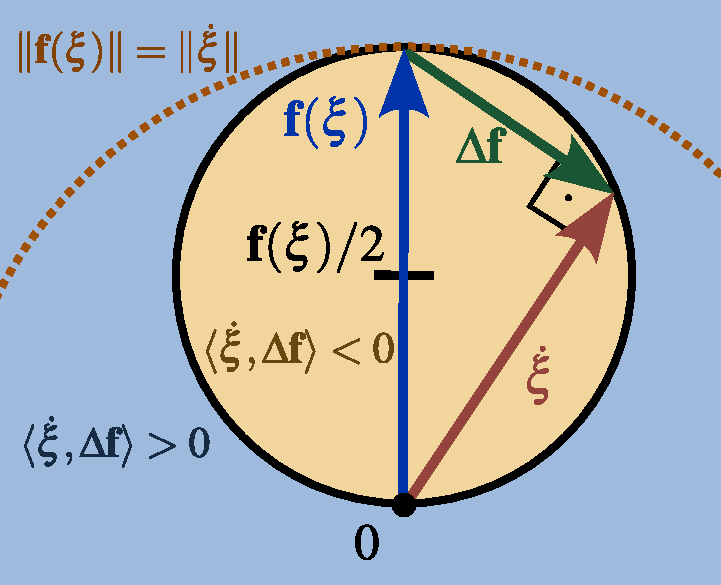
\includegraphics[width=0.7\columnwidth]{figures/passivity_analysis}
	\caption{The system is passive velocities $\dot{\vecs \xi}$ which are larger than the desired velocity $\vect f(\vecs \xi)$, i.e., outside the dashed orange circle.
    However, the system can be non-passive for small velocities, when  $\dotprod{\dot{\vecs \xi}}{\Delta \vect f} < 0$ (yellow circle). }
	\label{fig:passivity_analysis}
\end{figure}

\end{proof}

As in the red region, the system is not passive, the storage function $W$ could increase, and hence the velocity $\dot {\vecs \xi}$ could increase in a non-passive manner. This behavior is not unexpected, as the controller is designed to approach a desired DS $\vect{f}({\vecs \xi})$. Hence, as long as the desired velocity is not reached, the kinetic energy increases even with no force input $\vecs \tau^e$. While the passivity in Lemma~\ref{lemma:passivity}, only holds in a certain region. We can use this property to ensure the stability of the system:

\begin{theorem}  \label{theorem:passivity}
  Let $\vect f(\xi)$ is the desired velocity $\vect f(\vecs\xi)$ with bounded magnitude, i.e., $\| \vect f(\xi) \| < v^{\mathrm{max}}, \forall \xi \in \mathbb{R}^N$.
   The closed loop system \eqref{eq:robot_dynamics} is bounded-input, bounded-output (BIBO) stable using the controller from \eqref{eq:control_command} and damping matrix $\matd D(\vecs \xi)$ given in \eqref{eq:damping_summation} with respect to the input disturbance forces $\vect \tau^e$, and output the velocity $\dot{\vecs \xi}$.
\end{theorem}
 
\begin{proof}
From Lemma~\ref{lemma:passivity}, the system is passive when the magnitude of the velocity is larger than the dynamics, i.e. $\| \dot{\vecs \xi} \| > \|\vect f(\vecs \xi) \|$, the orange circle in Figure~\ref{fig:passivity_analysis}.
Inside this region, the system is not passive, and the velocity $\dot {\vecs \xi}$ can increase. However, the velocity increase is limited to staying below $\| \vect f({\vecs \xi}) \|$ before the system enters the region where it is passive. Hence, the control cannot introduce unexpected energy.
It follows that the system has a bounded output as long as the desired velocity $\mathbf{f}({\vecs \xi})$ is stable and the input $\int_{0}^T \dot{{\vecs \xi}}^T \vecs \tau^e dt$ is bounded. 
% Since as soon as the observed velocity $\| \dot{{\vecs \xi}} \| $ is larger than the desired velocity, the system behaves passively. Hence, the control cannot introduce unexpected energy.

% \subsubsection{Stability with General Damping}
From \eqref{eq:damping_summation}, a general damping matrix $\matd{S}(\vecs \xi)$ has non-uniform values. Hence, the analysis needs to be extended to general values.
The damping matrix $\matd{D}({\vecs \xi}) = \matd{Q}({\vecs \xi}) \matd{S}({\vecs \xi}) \matd{Q}({\vecs \xi})^{-1}$, can be interpreted as a coordinate transfer, such that:
\begin{equation}
	\vecs{\bar v} = \sqrt{\matd{S}({\vecs \xi})} \matd{Q}({\vecs \xi})^{-1} \dot{{\vecs \xi}}
	\quad \text{and} \quad
	\bar{\Delta \mathbf f} = \sqrt{\matd{S}({\vecs \xi})} \matd{Q}({\vecs \xi})^{-1} \Delta \mathbf{f}
\end{equation}
where the square root of the diagonal matrix $\Lambda({\vecs \xi})$ is taken element-wise:
\begin{equation}
\dot{\vecs \xi}^T \matd{D}({\vecs \xi}) \Delta \mathbf{f} = \vecs{\dot \xi}^T \matd{Q}({\vecs \xi}) \matd{S}({\vecs \xi}) \matd{Q}({\vecs \xi})^{-1} \Delta \mathbf{f} = \vecs{\bar v}^T \bar{\Delta \mathbf f}
\end{equation}
The analysis described in Fig.~\ref{fig:passivity_analysis} can hence be applied in the transformed space, too. 

For an orthogonal decomposition matrix $\matd{Q}(\boldsymbol{{\vecs \xi}})$, the region of non-passivity is an ellipse where the direction of the axes points along column vectors of $\matd{Q}({\vecs \xi})$, and the corresponding axes lengths are the diagonal elements of $\| \mathbf{f}({\vecs \xi})^T \sqrt{\matd{S}({\vecs \xi})}\| / 2 \sqrt{\matd{S}({\vecs \xi})}^{(-1)}$. 

If the axes' lengths are large, this can lead to accelerating the velocity even though it is already larger (but not pointing in the correct direction) than the desired velocity. However, the non-passive region is still bounded by an ellipse, and hence a maximum velocity.

While the passivity statement of Lemma~\ref{lemma:passivity} is local only, hence the controller can introduce energy into the system outside of the passive region. However, in such a case the system the velocity of the system increases and the system will enter the passive region system since it is bounded by a velocity limit.
However, passivity is used to prove that a controller does not \textit{pump} energy In that case, the controller acts passive and is ensured not to increase the system's energy anymore.
\end{proof}

This proof extends to a basis $\matd{Q}$, which is not orthogonal. However, in such a case, the controller must be carefully chosen to ensure that the speed up is limited when the basis is close to singular, for example by limiting the relative difference of the stretching vectors.

As stable behavior is ensured for a general shape of a damping matrix $\matd{D}$, the global stability proof extends to the general passive interaction control introduced in \cite{kronander2015passive}.

% Note, that in the case of $\langle e_2, e_n \rangle \neq 0$ the choice of $e_2$ does not matter as the corresponding  weight from \eqref{eq:eig2_weight} is $w_2 = 0$, hence it $\lambda_2 = \lambda$, as all eigenvalues.
